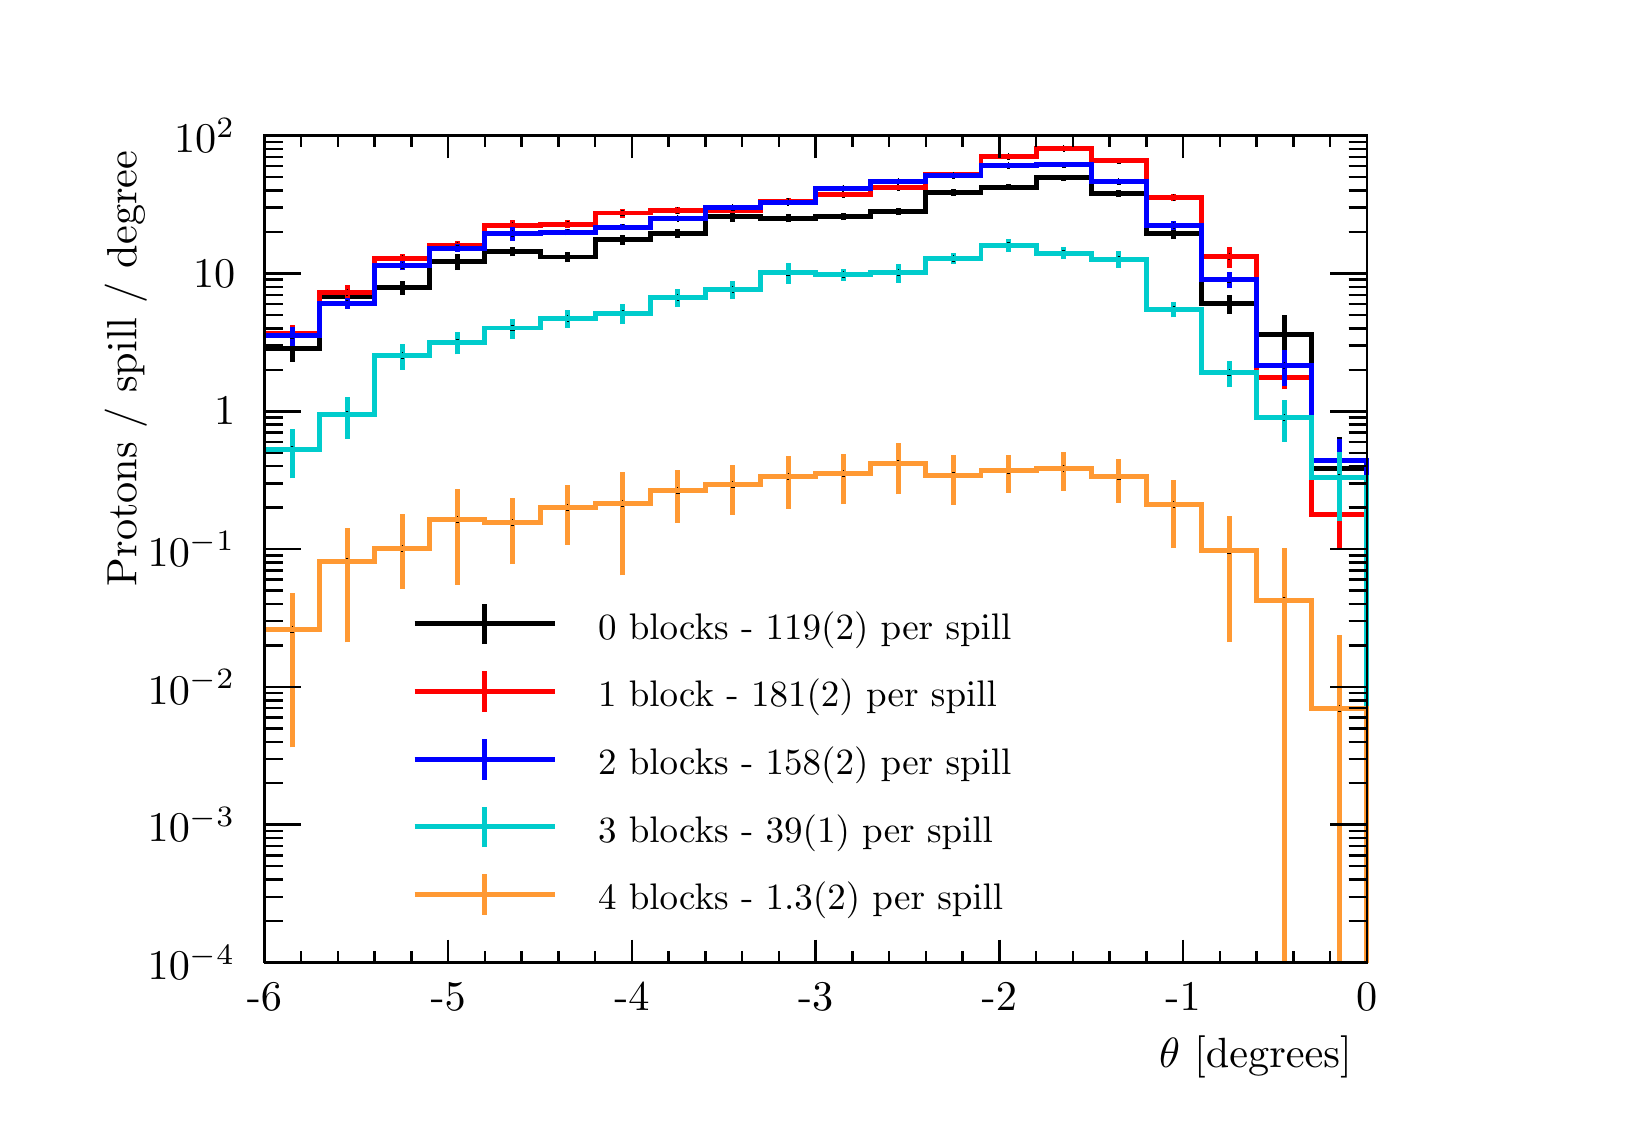
\begin{tikzpicture}
\pgfdeclareplotmark{cross} {
\pgfpathmoveto{\pgfpoint{-0.3\pgfplotmarksize}{\pgfplotmarksize}}
\pgfpathlineto{\pgfpoint{+0.3\pgfplotmarksize}{\pgfplotmarksize}}
\pgfpathlineto{\pgfpoint{+0.3\pgfplotmarksize}{0.3\pgfplotmarksize}}
\pgfpathlineto{\pgfpoint{+1\pgfplotmarksize}{0.3\pgfplotmarksize}}
\pgfpathlineto{\pgfpoint{+1\pgfplotmarksize}{-0.3\pgfplotmarksize}}
\pgfpathlineto{\pgfpoint{+0.3\pgfplotmarksize}{-0.3\pgfplotmarksize}}
\pgfpathlineto{\pgfpoint{+0.3\pgfplotmarksize}{-1.\pgfplotmarksize}}
\pgfpathlineto{\pgfpoint{-0.3\pgfplotmarksize}{-1.\pgfplotmarksize}}
\pgfpathlineto{\pgfpoint{-0.3\pgfplotmarksize}{-0.3\pgfplotmarksize}}
\pgfpathlineto{\pgfpoint{-1.\pgfplotmarksize}{-0.3\pgfplotmarksize}}
\pgfpathlineto{\pgfpoint{-1.\pgfplotmarksize}{0.3\pgfplotmarksize}}
\pgfpathlineto{\pgfpoint{-0.3\pgfplotmarksize}{0.3\pgfplotmarksize}}
\pgfpathclose
\pgfusepathqstroke
}
\pgfdeclareplotmark{cross*} {
\pgfpathmoveto{\pgfpoint{-0.3\pgfplotmarksize}{\pgfplotmarksize}}
\pgfpathlineto{\pgfpoint{+0.3\pgfplotmarksize}{\pgfplotmarksize}}
\pgfpathlineto{\pgfpoint{+0.3\pgfplotmarksize}{0.3\pgfplotmarksize}}
\pgfpathlineto{\pgfpoint{+1\pgfplotmarksize}{0.3\pgfplotmarksize}}
\pgfpathlineto{\pgfpoint{+1\pgfplotmarksize}{-0.3\pgfplotmarksize}}
\pgfpathlineto{\pgfpoint{+0.3\pgfplotmarksize}{-0.3\pgfplotmarksize}}
\pgfpathlineto{\pgfpoint{+0.3\pgfplotmarksize}{-1.\pgfplotmarksize}}
\pgfpathlineto{\pgfpoint{-0.3\pgfplotmarksize}{-1.\pgfplotmarksize}}
\pgfpathlineto{\pgfpoint{-0.3\pgfplotmarksize}{-0.3\pgfplotmarksize}}
\pgfpathlineto{\pgfpoint{-1.\pgfplotmarksize}{-0.3\pgfplotmarksize}}
\pgfpathlineto{\pgfpoint{-1.\pgfplotmarksize}{0.3\pgfplotmarksize}}
\pgfpathlineto{\pgfpoint{-0.3\pgfplotmarksize}{0.3\pgfplotmarksize}}
\pgfpathclose
\pgfusepathqfillstroke
}
\pgfdeclareplotmark{newstar} {
\pgfpathmoveto{\pgfqpoint{0pt}{\pgfplotmarksize}}
\pgfpathlineto{\pgfqpointpolar{44}{0.5\pgfplotmarksize}}
\pgfpathlineto{\pgfqpointpolar{18}{\pgfplotmarksize}}
\pgfpathlineto{\pgfqpointpolar{-20}{0.5\pgfplotmarksize}}
\pgfpathlineto{\pgfqpointpolar{-54}{\pgfplotmarksize}}
\pgfpathlineto{\pgfqpointpolar{-90}{0.5\pgfplotmarksize}}
\pgfpathlineto{\pgfqpointpolar{234}{\pgfplotmarksize}}
\pgfpathlineto{\pgfqpointpolar{198}{0.5\pgfplotmarksize}}
\pgfpathlineto{\pgfqpointpolar{162}{\pgfplotmarksize}}
\pgfpathlineto{\pgfqpointpolar{134}{0.5\pgfplotmarksize}}
\pgfpathclose
\pgfusepathqstroke
}
\pgfdeclareplotmark{newstar*} {
\pgfpathmoveto{\pgfqpoint{0pt}{\pgfplotmarksize}}
\pgfpathlineto{\pgfqpointpolar{44}{0.5\pgfplotmarksize}}
\pgfpathlineto{\pgfqpointpolar{18}{\pgfplotmarksize}}
\pgfpathlineto{\pgfqpointpolar{-20}{0.5\pgfplotmarksize}}
\pgfpathlineto{\pgfqpointpolar{-54}{\pgfplotmarksize}}
\pgfpathlineto{\pgfqpointpolar{-90}{0.5\pgfplotmarksize}}
\pgfpathlineto{\pgfqpointpolar{234}{\pgfplotmarksize}}
\pgfpathlineto{\pgfqpointpolar{198}{0.5\pgfplotmarksize}}
\pgfpathlineto{\pgfqpointpolar{162}{\pgfplotmarksize}}
\pgfpathlineto{\pgfqpointpolar{134}{0.5\pgfplotmarksize}}
\pgfpathclose
\pgfusepathqfillstroke
}
\definecolor{c}{rgb}{1,1,1};
\draw [color=c, fill=c] (0,0) rectangle (20,13.639);
\draw [color=c, fill=c] (3,1.77307) rectangle (17,12.2751);
\definecolor{c}{rgb}{0,0,0};
\draw [c,line width=0.9] (3,1.77307) -- (3,12.2751) -- (17,12.2751) -- (17,1.77307) -- (3,1.77307);
\definecolor{c}{rgb}{1,1,1};
\draw [color=c, fill=c] (3,1.77307) rectangle (17,12.2751);
\definecolor{c}{rgb}{0,0,0};
\draw [c,line width=0.9] (3,1.77307) -- (3,12.2751) -- (17,12.2751) -- (17,1.77307) -- (3,1.77307);
\draw [c,line width=0.9] (3,1.77307) -- (3.7,1.77307) -- (3.7,1.77307) -- (4.4,1.77307) -- (4.4,1.77307) -- (5.1,1.77307) -- (5.1,1.77307) -- (5.8,1.77307) -- (5.8,1.77307) -- (6.5,1.77307) -- (6.5,1.77307) -- (7.2,1.77307) -- (7.2,1.77307) --
 (7.9,1.77307) -- (7.9,1.77307) -- (8.6,1.77307) -- (8.6,1.77307) -- (9.3,1.77307) -- (9.3,1.77307) -- (10,1.77307) -- (10,1.77307) -- (10.7,1.77307) -- (10.7,1.77307) -- (11.4,1.77307) -- (11.4,1.77307) -- (12.1,1.77307) -- (12.1,1.77307) --
 (12.8,1.77307) -- (12.8,1.77307) -- (13.5,1.77307) -- (13.5,1.77307) -- (14.2,1.77307) -- (14.2,1.77307) -- (14.9,1.77307) -- (14.9,1.77307) -- (15.6,1.77307) -- (15.6,1.77307) -- (16.3,1.77307) -- (16.3,1.77307) -- (17,1.77307) -- (17,1.77307);
\draw [c,line width=0.9] (3,1.77307) -- (17,1.77307);
\draw [c,line width=0.9] (3,2.05948) -- (3,1.77307);
\draw [c,line width=0.9] (3.46667,1.91628) -- (3.46667,1.77307);
\draw [c,line width=0.9] (3.93333,1.91628) -- (3.93333,1.77307);
\draw [c,line width=0.9] (4.4,1.91628) -- (4.4,1.77307);
\draw [c,line width=0.9] (4.86667,1.91628) -- (4.86667,1.77307);
\draw [c,line width=0.9] (5.33333,2.05948) -- (5.33333,1.77307);
\draw [c,line width=0.9] (5.8,1.91628) -- (5.8,1.77307);
\draw [c,line width=0.9] (6.26667,1.91628) -- (6.26667,1.77307);
\draw [c,line width=0.9] (6.73333,1.91628) -- (6.73333,1.77307);
\draw [c,line width=0.9] (7.2,1.91628) -- (7.2,1.77307);
\draw [c,line width=0.9] (7.66667,2.05948) -- (7.66667,1.77307);
\draw [c,line width=0.9] (8.13333,1.91628) -- (8.13333,1.77307);
\draw [c,line width=0.9] (8.6,1.91628) -- (8.6,1.77307);
\draw [c,line width=0.9] (9.06667,1.91628) -- (9.06667,1.77307);
\draw [c,line width=0.9] (9.53333,1.91628) -- (9.53333,1.77307);
\draw [c,line width=0.9] (10,2.05948) -- (10,1.77307);
\draw [c,line width=0.9] (10.4667,1.91628) -- (10.4667,1.77307);
\draw [c,line width=0.9] (10.9333,1.91628) -- (10.9333,1.77307);
\draw [c,line width=0.9] (11.4,1.91628) -- (11.4,1.77307);
\draw [c,line width=0.9] (11.8667,1.91628) -- (11.8667,1.77307);
\draw [c,line width=0.9] (12.3333,2.05948) -- (12.3333,1.77307);
\draw [c,line width=0.9] (12.8,1.91628) -- (12.8,1.77307);
\draw [c,line width=0.9] (13.2667,1.91628) -- (13.2667,1.77307);
\draw [c,line width=0.9] (13.7333,1.91628) -- (13.7333,1.77307);
\draw [c,line width=0.9] (14.2,1.91628) -- (14.2,1.77307);
\draw [c,line width=0.9] (14.6667,2.05948) -- (14.6667,1.77307);
\draw [c,line width=0.9] (15.1333,1.91628) -- (15.1333,1.77307);
\draw [c,line width=0.9] (15.6,1.91628) -- (15.6,1.77307);
\draw [c,line width=0.9] (16.0667,1.91628) -- (16.0667,1.77307);
\draw [c,line width=0.9] (16.5333,1.91628) -- (16.5333,1.77307);
\draw [c,line width=0.9] (17,2.05948) -- (17,1.77307);
\draw [anchor=base] (3,1.15931) node[scale=1.52731, color=c, rotate=0]{-6};
\draw [anchor=base] (5.33333,1.15931) node[scale=1.52731, color=c, rotate=0]{-5};
\draw [anchor=base] (7.66667,1.15931) node[scale=1.52731, color=c, rotate=0]{-4};
\draw [anchor=base] (10,1.15931) node[scale=1.52731, color=c, rotate=0]{-3};
\draw [anchor=base] (12.3333,1.15931) node[scale=1.52731, color=c, rotate=0]{-2};
\draw [anchor=base] (14.6667,1.15931) node[scale=1.52731, color=c, rotate=0]{-1};
\draw [anchor=base] (17,1.15931) node[scale=1.52731, color=c, rotate=0]{0};
\draw [anchor= east] (17,0.572837) node[scale=1.52731, color=c, rotate=0]{$\theta$  [degrees]};
\draw [c,line width=0.9] (3,12.2751) -- (17,12.2751);
\draw [c,line width=0.9] (3,11.9887) -- (3,12.2751);
\draw [c,line width=0.9] (3.46667,12.1319) -- (3.46667,12.2751);
\draw [c,line width=0.9] (3.93333,12.1319) -- (3.93333,12.2751);
\draw [c,line width=0.9] (4.4,12.1319) -- (4.4,12.2751);
\draw [c,line width=0.9] (4.86667,12.1319) -- (4.86667,12.2751);
\draw [c,line width=0.9] (5.33333,11.9887) -- (5.33333,12.2751);
\draw [c,line width=0.9] (5.8,12.1319) -- (5.8,12.2751);
\draw [c,line width=0.9] (6.26667,12.1319) -- (6.26667,12.2751);
\draw [c,line width=0.9] (6.73333,12.1319) -- (6.73333,12.2751);
\draw [c,line width=0.9] (7.2,12.1319) -- (7.2,12.2751);
\draw [c,line width=0.9] (7.66667,11.9887) -- (7.66667,12.2751);
\draw [c,line width=0.9] (8.13333,12.1319) -- (8.13333,12.2751);
\draw [c,line width=0.9] (8.6,12.1319) -- (8.6,12.2751);
\draw [c,line width=0.9] (9.06667,12.1319) -- (9.06667,12.2751);
\draw [c,line width=0.9] (9.53333,12.1319) -- (9.53333,12.2751);
\draw [c,line width=0.9] (10,11.9887) -- (10,12.2751);
\draw [c,line width=0.9] (10.4667,12.1319) -- (10.4667,12.2751);
\draw [c,line width=0.9] (10.9333,12.1319) -- (10.9333,12.2751);
\draw [c,line width=0.9] (11.4,12.1319) -- (11.4,12.2751);
\draw [c,line width=0.9] (11.8667,12.1319) -- (11.8667,12.2751);
\draw [c,line width=0.9] (12.3333,11.9887) -- (12.3333,12.2751);
\draw [c,line width=0.9] (12.8,12.1319) -- (12.8,12.2751);
\draw [c,line width=0.9] (13.2667,12.1319) -- (13.2667,12.2751);
\draw [c,line width=0.9] (13.7333,12.1319) -- (13.7333,12.2751);
\draw [c,line width=0.9] (14.2,12.1319) -- (14.2,12.2751);
\draw [c,line width=0.9] (14.6667,11.9887) -- (14.6667,12.2751);
\draw [c,line width=0.9] (15.1333,12.1319) -- (15.1333,12.2751);
\draw [c,line width=0.9] (15.6,12.1319) -- (15.6,12.2751);
\draw [c,line width=0.9] (16.0667,12.1319) -- (16.0667,12.2751);
\draw [c,line width=0.9] (16.5333,12.1319) -- (16.5333,12.2751);
\draw [c,line width=0.9] (17,11.9887) -- (17,12.2751);
\draw [c,line width=0.9] (3,1.77307) -- (3,12.2751);
\draw [c,line width=0.9] (3.462,1.77307) -- (3,1.77307);
\draw [anchor= east] (2.82,1.77307) node[scale=1.52731, color=c, rotate=0]{$10^{-4}$};
\draw [c,line width=0.9] (3.231,2.29997) -- (3,2.29997);
\draw [c,line width=0.9] (3.231,2.60819) -- (3,2.60819);
\draw [c,line width=0.9] (3.231,2.82687) -- (3,2.82687);
\draw [c,line width=0.9] (3.231,2.9965) -- (3,2.9965);
\draw [c,line width=0.9] (3.231,3.13509) -- (3,3.13509);
\draw [c,line width=0.9] (3.231,3.25227) -- (3,3.25227);
\draw [c,line width=0.9] (3.231,3.35378) -- (3,3.35378);
\draw [c,line width=0.9] (3.231,3.44331) -- (3,3.44331);
\draw [c,line width=0.9] (3.462,3.5234) -- (3,3.5234);
\draw [anchor= east] (2.82,3.5234) node[scale=1.52731, color=c, rotate=0]{$10^{-3}$};
\draw [c,line width=0.9] (3.231,4.0503) -- (3,4.0503);
\draw [c,line width=0.9] (3.231,4.35852) -- (3,4.35852);
\draw [c,line width=0.9] (3.231,4.57721) -- (3,4.57721);
\draw [c,line width=0.9] (3.231,4.74683) -- (3,4.74683);
\draw [c,line width=0.9] (3.231,4.88543) -- (3,4.88543);
\draw [c,line width=0.9] (3.231,5.00261) -- (3,5.00261);
\draw [c,line width=0.9] (3.231,5.10411) -- (3,5.10411);
\draw [c,line width=0.9] (3.231,5.19364) -- (3,5.19364);
\draw [c,line width=0.9] (3.462,5.27374) -- (3,5.27374);
\draw [anchor= east] (2.82,5.27374) node[scale=1.52731, color=c, rotate=0]{$10^{-2}$};
\draw [c,line width=0.9] (3.231,5.80064) -- (3,5.80064);
\draw [c,line width=0.9] (3.231,6.10886) -- (3,6.10886);
\draw [c,line width=0.9] (3.231,6.32754) -- (3,6.32754);
\draw [c,line width=0.9] (3.231,6.49717) -- (3,6.49717);
\draw [c,line width=0.9] (3.231,6.63576) -- (3,6.63576);
\draw [c,line width=0.9] (3.231,6.75294) -- (3,6.75294);
\draw [c,line width=0.9] (3.231,6.85444) -- (3,6.85444);
\draw [c,line width=0.9] (3.231,6.94398) -- (3,6.94398);
\draw [c,line width=0.9] (3.462,7.02407) -- (3,7.02407);
\draw [anchor= east] (2.82,7.02407) node[scale=1.52731, color=c, rotate=0]{$10^{-1}$};
\draw [c,line width=0.9] (3.231,7.55097) -- (3,7.55097);
\draw [c,line width=0.9] (3.231,7.85919) -- (3,7.85919);
\draw [c,line width=0.9] (3.231,8.07788) -- (3,8.07788);
\draw [c,line width=0.9] (3.231,8.2475) -- (3,8.2475);
\draw [c,line width=0.9] (3.231,8.38609) -- (3,8.38609);
\draw [c,line width=0.9] (3.231,8.50327) -- (3,8.50327);
\draw [c,line width=0.9] (3.231,8.60478) -- (3,8.60478);
\draw [c,line width=0.9] (3.231,8.69431) -- (3,8.69431);
\draw [c,line width=0.9] (3.462,8.7744) -- (3,8.7744);
\draw [anchor= east] (2.82,8.7744) node[scale=1.52731, color=c, rotate=0]{1};
\draw [c,line width=0.9] (3.231,9.30131) -- (3,9.30131);
\draw [c,line width=0.9] (3.231,9.60952) -- (3,9.60952);
\draw [c,line width=0.9] (3.231,9.82821) -- (3,9.82821);
\draw [c,line width=0.9] (3.231,9.99783) -- (3,9.99783);
\draw [c,line width=0.9] (3.231,10.1364) -- (3,10.1364);
\draw [c,line width=0.9] (3.231,10.2536) -- (3,10.2536);
\draw [c,line width=0.9] (3.231,10.3551) -- (3,10.3551);
\draw [c,line width=0.9] (3.231,10.4446) -- (3,10.4446);
\draw [c,line width=0.9] (3.462,10.5247) -- (3,10.5247);
\draw [anchor= east] (2.82,10.5247) node[scale=1.52731, color=c, rotate=0]{10};
\draw [c,line width=0.9] (3.231,11.0516) -- (3,11.0516);
\draw [c,line width=0.9] (3.231,11.3599) -- (3,11.3599);
\draw [c,line width=0.9] (3.231,11.5785) -- (3,11.5785);
\draw [c,line width=0.9] (3.231,11.7482) -- (3,11.7482);
\draw [c,line width=0.9] (3.231,11.8868) -- (3,11.8868);
\draw [c,line width=0.9] (3.231,12.0039) -- (3,12.0039);
\draw [c,line width=0.9] (3.231,12.1054) -- (3,12.1054);
\draw [c,line width=0.9] (3.231,12.195) -- (3,12.195);
\draw [c,line width=0.9] (3.462,12.2751) -- (3,12.2751);
\draw [anchor= east] (2.82,12.2751) node[scale=1.52731, color=c, rotate=0]{$10^{2}$};
\draw [anchor= east] (1.24,12.2751) node[scale=1.52731, color=c, rotate=90]{ Protons / spill / degree};
\draw [c,line width=0.9] (17,1.77307) -- (17,12.2751);
\draw [c,line width=0.9] (16.538,1.77307) -- (17,1.77307);
\draw [c,line width=0.9] (16.769,2.29997) -- (17,2.29997);
\draw [c,line width=0.9] (16.769,2.60819) -- (17,2.60819);
\draw [c,line width=0.9] (16.769,2.82687) -- (17,2.82687);
\draw [c,line width=0.9] (16.769,2.9965) -- (17,2.9965);
\draw [c,line width=0.9] (16.769,3.13509) -- (17,3.13509);
\draw [c,line width=0.9] (16.769,3.25227) -- (17,3.25227);
\draw [c,line width=0.9] (16.769,3.35378) -- (17,3.35378);
\draw [c,line width=0.9] (16.769,3.44331) -- (17,3.44331);
\draw [c,line width=0.9] (16.538,3.5234) -- (17,3.5234);
\draw [c,line width=0.9] (16.769,4.0503) -- (17,4.0503);
\draw [c,line width=0.9] (16.769,4.35852) -- (17,4.35852);
\draw [c,line width=0.9] (16.769,4.57721) -- (17,4.57721);
\draw [c,line width=0.9] (16.769,4.74683) -- (17,4.74683);
\draw [c,line width=0.9] (16.769,4.88543) -- (17,4.88543);
\draw [c,line width=0.9] (16.769,5.00261) -- (17,5.00261);
\draw [c,line width=0.9] (16.769,5.10411) -- (17,5.10411);
\draw [c,line width=0.9] (16.769,5.19364) -- (17,5.19364);
\draw [c,line width=0.9] (16.538,5.27374) -- (17,5.27374);
\draw [c,line width=0.9] (16.769,5.80064) -- (17,5.80064);
\draw [c,line width=0.9] (16.769,6.10886) -- (17,6.10886);
\draw [c,line width=0.9] (16.769,6.32754) -- (17,6.32754);
\draw [c,line width=0.9] (16.769,6.49717) -- (17,6.49717);
\draw [c,line width=0.9] (16.769,6.63576) -- (17,6.63576);
\draw [c,line width=0.9] (16.769,6.75294) -- (17,6.75294);
\draw [c,line width=0.9] (16.769,6.85444) -- (17,6.85444);
\draw [c,line width=0.9] (16.769,6.94398) -- (17,6.94398);
\draw [c,line width=0.9] (16.538,7.02407) -- (17,7.02407);
\draw [c,line width=0.9] (16.769,7.55097) -- (17,7.55097);
\draw [c,line width=0.9] (16.769,7.85919) -- (17,7.85919);
\draw [c,line width=0.9] (16.769,8.07788) -- (17,8.07788);
\draw [c,line width=0.9] (16.769,8.2475) -- (17,8.2475);
\draw [c,line width=0.9] (16.769,8.38609) -- (17,8.38609);
\draw [c,line width=0.9] (16.769,8.50327) -- (17,8.50327);
\draw [c,line width=0.9] (16.769,8.60478) -- (17,8.60478);
\draw [c,line width=0.9] (16.769,8.69431) -- (17,8.69431);
\draw [c,line width=0.9] (16.538,8.7744) -- (17,8.7744);
\draw [c,line width=0.9] (16.769,9.30131) -- (17,9.30131);
\draw [c,line width=0.9] (16.769,9.60952) -- (17,9.60952);
\draw [c,line width=0.9] (16.769,9.82821) -- (17,9.82821);
\draw [c,line width=0.9] (16.769,9.99783) -- (17,9.99783);
\draw [c,line width=0.9] (16.769,10.1364) -- (17,10.1364);
\draw [c,line width=0.9] (16.769,10.2536) -- (17,10.2536);
\draw [c,line width=0.9] (16.769,10.3551) -- (17,10.3551);
\draw [c,line width=0.9] (16.769,10.4446) -- (17,10.4446);
\draw [c,line width=0.9] (16.538,10.5247) -- (17,10.5247);
\draw [c,line width=0.9] (16.769,11.0516) -- (17,11.0516);
\draw [c,line width=0.9] (16.769,11.3599) -- (17,11.3599);
\draw [c,line width=0.9] (16.769,11.5785) -- (17,11.5785);
\draw [c,line width=0.9] (16.769,11.7482) -- (17,11.7482);
\draw [c,line width=0.9] (16.769,11.8868) -- (17,11.8868);
\draw [c,line width=0.9] (16.769,12.0039) -- (17,12.0039);
\draw [c,line width=0.9] (16.769,12.1054) -- (17,12.1054);
\draw [c,line width=0.9] (16.769,12.195) -- (17,12.195);
\draw [c,line width=0.9] (16.538,12.2751) -- (17,12.2751);
\draw [c,line width=1.8] (3.35,9.40045) -- (3.35,9.56717);
\draw [c,line width=1.8] (3.35,9.56717) -- (3.35,9.70383);
\foreach \P in {(3.35,9.56717)}{\draw[mark options={color=c,fill=c},mark size=2.402402pt, line width=0.000000pt, mark=*,mark size=1pt] plot coordinates {\P};}
\draw [c,line width=1.8] (4.05,10.127) -- (4.05,10.2259);
\draw [c,line width=1.8] (4.05,10.2259) -- (4.05,10.3134);
\foreach \P in {(4.05,10.2259)}{\draw[mark options={color=c,fill=c},mark size=2.402402pt, line width=0.000000pt, mark=*,mark size=1pt] plot coordinates {\P};}
\draw [c,line width=1.8] (4.75,10.2513) -- (4.75,10.3438);
\draw [c,line width=1.8] (4.75,10.3438) -- (4.75,10.4262);
\foreach \P in {(4.75,10.3438)}{\draw[mark options={color=c,fill=c},mark size=2.402402pt, line width=0.000000pt, mark=*,mark size=1pt] plot coordinates {\P};}
\draw [c,line width=1.8] (5.45,10.5652) -- (5.45,10.6779);
\draw [c,line width=1.8] (5.45,10.6779) -- (5.45,10.776);
\foreach \P in {(5.45,10.6779)}{\draw[mark options={color=c,fill=c},mark size=2.402402pt, line width=0.000000pt, mark=*,mark size=1pt] plot coordinates {\P};}
\draw [c,line width=1.8] (6.15,10.74) -- (6.15,10.8057);
\draw [c,line width=1.8] (6.15,10.8057) -- (6.15,10.8662);
\foreach \P in {(6.15,10.8057)}{\draw[mark options={color=c,fill=c},mark size=2.402402pt, line width=0.000000pt, mark=*,mark size=1pt] plot coordinates {\P};}
\draw [c,line width=1.8] (6.85,10.664) -- (6.85,10.7334);
\draw [c,line width=1.8] (6.85,10.7334) -- (6.85,10.7971);
\foreach \P in {(6.85,10.7334)}{\draw[mark options={color=c,fill=c},mark size=2.402402pt, line width=0.000000pt, mark=*,mark size=1pt] plot coordinates {\P};}
\draw [c,line width=1.8] (7.55,10.8875) -- (7.55,10.9524);
\draw [c,line width=1.8] (7.55,10.9524) -- (7.55,11.0122);
\foreach \P in {(7.55,10.9524)}{\draw[mark options={color=c,fill=c},mark size=2.402402pt, line width=0.000000pt, mark=*,mark size=1pt] plot coordinates {\P};}
\draw [c,line width=1.8] (8.25,10.9728) -- (8.25,11.0311);
\draw [c,line width=1.8] (8.25,11.0311) -- (8.25,11.0852);
\foreach \P in {(8.25,11.0311)}{\draw[mark options={color=c,fill=c},mark size=2.402402pt, line width=0.000000pt, mark=*,mark size=1pt] plot coordinates {\P};}
\draw [c,line width=1.8] (8.95,11.1783) -- (8.95,11.246);
\draw [c,line width=1.8] (8.95,11.246) -- (8.95,11.3081);
\foreach \P in {(8.95,11.246)}{\draw[mark options={color=c,fill=c},mark size=2.402402pt, line width=0.000000pt, mark=*,mark size=1pt] plot coordinates {\P};}
\draw [c,line width=1.8] (9.65,11.1747) -- (9.65,11.2272);
\draw [c,line width=1.8] (9.65,11.2272) -- (9.65,11.2762);
\foreach \P in {(9.65,11.2272)}{\draw[mark options={color=c,fill=c},mark size=2.402402pt, line width=0.000000pt, mark=*,mark size=1pt] plot coordinates {\P};}
\draw [c,line width=1.8] (10.35,11.203) -- (10.35,11.2513);
\draw [c,line width=1.8] (10.35,11.2513) -- (10.35,11.2967);
\foreach \P in {(10.35,11.2513)}{\draw[mark options={color=c,fill=c},mark size=2.402402pt, line width=0.000000pt, mark=*,mark size=1pt] plot coordinates {\P};}
\draw [c,line width=1.8] (11.05,11.2668) -- (11.05,11.3128);
\draw [c,line width=1.8] (11.05,11.3128) -- (11.05,11.3562);
\foreach \P in {(11.05,11.3128)}{\draw[mark options={color=c,fill=c},mark size=2.402402pt, line width=0.000000pt, mark=*,mark size=1pt] plot coordinates {\P};}
\draw [c,line width=1.8] (11.75,11.5097) -- (11.75,11.5543);
\draw [c,line width=1.8] (11.75,11.5543) -- (11.75,11.5965);
\foreach \P in {(11.75,11.5543)}{\draw[mark options={color=c,fill=c},mark size=2.402402pt, line width=0.000000pt, mark=*,mark size=1pt] plot coordinates {\P};}
\draw [c,line width=1.8] (12.45,11.5854) -- (12.45,11.6211);
\draw [c,line width=1.8] (12.45,11.6211) -- (12.45,11.6551);
\foreach \P in {(12.45,11.6211)}{\draw[mark options={color=c,fill=c},mark size=2.402402pt, line width=0.000000pt, mark=*,mark size=1pt] plot coordinates {\P};}
\draw [c,line width=1.8] (13.15,11.7045) -- (13.15,11.7389);
\draw [c,line width=1.8] (13.15,11.7389) -- (13.15,11.7718);
\foreach \P in {(13.15,11.7389)}{\draw[mark options={color=c,fill=c},mark size=2.402402pt, line width=0.000000pt, mark=*,mark size=1pt] plot coordinates {\P};}
\draw [c,line width=1.8] (13.85,11.4945) -- (13.85,11.5401);
\draw [c,line width=1.8] (13.85,11.5401) -- (13.85,11.583);
\foreach \P in {(13.85,11.5401)}{\draw[mark options={color=c,fill=c},mark size=2.402402pt, line width=0.000000pt, mark=*,mark size=1pt] plot coordinates {\P};}
\draw [c,line width=1.8] (14.55,10.9603) -- (14.55,11.0273);
\draw [c,line width=1.8] (14.55,11.0273) -- (14.55,11.0888);
\foreach \P in {(14.55,11.0273)}{\draw[mark options={color=c,fill=c},mark size=2.402402pt, line width=0.000000pt, mark=*,mark size=1pt] plot coordinates {\P};}
\draw [c,line width=1.8] (15.25,10.0076) -- (15.25,10.1415);
\draw [c,line width=1.8] (15.25,10.1415) -- (15.25,10.2553);
\foreach \P in {(15.25,10.1415)}{\draw[mark options={color=c,fill=c},mark size=2.402402pt, line width=0.000000pt, mark=*,mark size=1pt] plot coordinates {\P};}
\draw [c,line width=1.8] (15.95,9.37851) -- (15.95,9.74619);
\draw [c,line width=1.8] (15.95,9.74619) -- (15.95,9.99294);
\foreach \P in {(15.95,9.74619)}{\draw[mark options={color=c,fill=c},mark size=2.402402pt, line width=0.000000pt, mark=*,mark size=1pt] plot coordinates {\P};}
\draw [c,line width=1.8] (16.65,7.08272) -- (16.65,8.04157);
\draw [c,line width=1.8] (16.65,8.04157) -- (16.65,8.45238);
\foreach \P in {(16.65,8.04157)}{\draw[mark options={color=c,fill=c},mark size=2.402402pt, line width=0.000000pt, mark=*,mark size=1pt] plot coordinates {\P};}
\draw [c,line width=1.8] (3,9.56717) -- (3.7,9.56717) -- (3.7,10.2259) -- (4.4,10.2259) -- (4.4,10.3438) -- (5.1,10.3438) -- (5.1,10.6779) -- (5.8,10.6779) -- (5.8,10.8057) -- (6.5,10.8057) -- (6.5,10.7334) -- (7.2,10.7334) -- (7.2,10.9524) --
 (7.9,10.9524) -- (7.9,11.0311) -- (8.6,11.0311) -- (8.6,11.246) -- (9.3,11.246) -- (9.3,11.2272) -- (10,11.2272) -- (10,11.2513) -- (10.7,11.2513) -- (10.7,11.3128) -- (11.4,11.3128) -- (11.4,11.5543) -- (12.1,11.5543) -- (12.1,11.6211) --
 (12.8,11.6211) -- (12.8,11.7389) -- (13.5,11.7389) -- (13.5,11.5401) -- (14.2,11.5401) -- (14.2,11.0273) -- (14.9,11.0273) -- (14.9,10.1415) -- (15.6,10.1415) -- (15.6,9.74619) -- (16.3,9.74619) -- (16.3,8.04157) -- (17,8.04157) -- (17,1.77307);
\definecolor{c}{rgb}{1,0,0};
\draw [c,line width=1.8] (3.35,9.63197) -- (3.35,9.76121);
\draw [c,line width=1.8] (3.35,9.76121) -- (3.35,9.87164);
\definecolor{c}{rgb}{0,0,0};
\foreach \P in {(3.35,9.76121)}{\draw[mark options={color=c,fill=c},mark size=2.402402pt, line width=0.000000pt, mark=*,mark size=1pt] plot coordinates {\P};}
\definecolor{c}{rgb}{1,0,0};
\draw [c,line width=1.8] (4.05,10.1749) -- (4.05,10.2836);
\draw [c,line width=1.8] (4.05,10.2836) -- (4.05,10.3787);
\definecolor{c}{rgb}{0,0,0};
\foreach \P in {(4.05,10.2836)}{\draw[mark options={color=c,fill=c},mark size=2.402402pt, line width=0.000000pt, mark=*,mark size=1pt] plot coordinates {\P};}
\definecolor{c}{rgb}{1,0,0};
\draw [c,line width=1.8] (4.75,10.6463) -- (4.75,10.7119);
\draw [c,line width=1.8] (4.75,10.7119) -- (4.75,10.7722);
\definecolor{c}{rgb}{0,0,0};
\foreach \P in {(4.75,10.7119)}{\draw[mark options={color=c,fill=c},mark size=2.402402pt, line width=0.000000pt, mark=*,mark size=1pt] plot coordinates {\P};}
\definecolor{c}{rgb}{1,0,0};
\draw [c,line width=1.8] (5.45,10.83) -- (5.45,10.8832);
\draw [c,line width=1.8] (5.45,10.8832) -- (5.45,10.933);
\definecolor{c}{rgb}{0,0,0};
\foreach \P in {(5.45,10.8832)}{\draw[mark options={color=c,fill=c},mark size=2.402402pt, line width=0.000000pt, mark=*,mark size=1pt] plot coordinates {\P};}
\definecolor{c}{rgb}{1,0,0};
\draw [c,line width=1.8] (6.15,11.0534) -- (6.15,11.1307);
\draw [c,line width=1.8] (6.15,11.1307) -- (6.15,11.2009);
\definecolor{c}{rgb}{0,0,0};
\foreach \P in {(6.15,11.1307)}{\draw[mark options={color=c,fill=c},mark size=2.402402pt, line width=0.000000pt, mark=*,mark size=1pt] plot coordinates {\P};}
\definecolor{c}{rgb}{1,0,0};
\draw [c,line width=1.8] (6.85,11.0977) -- (6.85,11.1503);
\draw [c,line width=1.8] (6.85,11.1503) -- (6.85,11.1994);
\definecolor{c}{rgb}{0,0,0};
\foreach \P in {(6.85,11.1503)}{\draw[mark options={color=c,fill=c},mark size=2.402402pt, line width=0.000000pt, mark=*,mark size=1pt] plot coordinates {\P};}
\definecolor{c}{rgb}{1,0,0};
\draw [c,line width=1.8] (7.55,11.2338) -- (7.55,11.2922);
\draw [c,line width=1.8] (7.55,11.2922) -- (7.55,11.3464);
\definecolor{c}{rgb}{0,0,0};
\foreach \P in {(7.55,11.2922)}{\draw[mark options={color=c,fill=c},mark size=2.402402pt, line width=0.000000pt, mark=*,mark size=1pt] plot coordinates {\P};}
\definecolor{c}{rgb}{1,0,0};
\draw [c,line width=1.8] (8.25,11.2764) -- (8.25,11.3225);
\draw [c,line width=1.8] (8.25,11.3225) -- (8.25,11.3661);
\definecolor{c}{rgb}{0,0,0};
\foreach \P in {(8.25,11.3225)}{\draw[mark options={color=c,fill=c},mark size=2.402402pt, line width=0.000000pt, mark=*,mark size=1pt] plot coordinates {\P};}
\definecolor{c}{rgb}{1,0,0};
\draw [c,line width=1.8] (8.95,11.2927) -- (8.95,11.3279);
\draw [c,line width=1.8] (8.95,11.3279) -- (8.95,11.3616);
\definecolor{c}{rgb}{0,0,0};
\foreach \P in {(8.95,11.3279)}{\draw[mark options={color=c,fill=c},mark size=2.402402pt, line width=0.000000pt, mark=*,mark size=1pt] plot coordinates {\P};}
\definecolor{c}{rgb}{1,0,0};
\draw [c,line width=1.8] (9.65,11.407) -- (9.65,11.4441);
\draw [c,line width=1.8] (9.65,11.4441) -- (9.65,11.4795);
\definecolor{c}{rgb}{0,0,0};
\foreach \P in {(9.65,11.4441)}{\draw[mark options={color=c,fill=c},mark size=2.402402pt, line width=0.000000pt, mark=*,mark size=1pt] plot coordinates {\P};}
\definecolor{c}{rgb}{1,0,0};
\draw [c,line width=1.8] (10.35,11.4894) -- (10.35,11.5258);
\draw [c,line width=1.8] (10.35,11.5258) -- (10.35,11.5605);
\definecolor{c}{rgb}{0,0,0};
\foreach \P in {(10.35,11.5258)}{\draw[mark options={color=c,fill=c},mark size=2.402402pt, line width=0.000000pt, mark=*,mark size=1pt] plot coordinates {\P};}
\definecolor{c}{rgb}{1,0,0};
\draw [c,line width=1.8] (11.05,11.5835) -- (11.05,11.6147);
\draw [c,line width=1.8] (11.05,11.6147) -- (11.05,11.6447);
\definecolor{c}{rgb}{0,0,0};
\foreach \P in {(11.05,11.6147)}{\draw[mark options={color=c,fill=c},mark size=2.402402pt, line width=0.000000pt, mark=*,mark size=1pt] plot coordinates {\P};}
\definecolor{c}{rgb}{1,0,0};
\draw [c,line width=1.8] (11.75,11.7475) -- (11.75,11.7777);
\draw [c,line width=1.8] (11.75,11.7777) -- (11.75,11.8067);
\definecolor{c}{rgb}{0,0,0};
\foreach \P in {(11.75,11.7777)}{\draw[mark options={color=c,fill=c},mark size=2.402402pt, line width=0.000000pt, mark=*,mark size=1pt] plot coordinates {\P};}
\definecolor{c}{rgb}{1,0,0};
\draw [c,line width=1.8] (12.45,11.987) -- (12.45,12.0102);
\draw [c,line width=1.8] (12.45,12.0102) -- (12.45,12.0327);
\definecolor{c}{rgb}{0,0,0};
\foreach \P in {(12.45,12.0102)}{\draw[mark options={color=c,fill=c},mark size=2.402402pt, line width=0.000000pt, mark=*,mark size=1pt] plot coordinates {\P};}
\definecolor{c}{rgb}{1,0,0};
\draw [c,line width=1.8] (13.15,12.0823) -- (13.15,12.1117);
\draw [c,line width=1.8] (13.15,12.1117) -- (13.15,12.14);
\definecolor{c}{rgb}{0,0,0};
\foreach \P in {(13.15,12.1117)}{\draw[mark options={color=c,fill=c},mark size=2.402402pt, line width=0.000000pt, mark=*,mark size=1pt] plot coordinates {\P};}
\definecolor{c}{rgb}{1,0,0};
\draw [c,line width=1.8] (13.85,11.9229) -- (13.85,11.9544);
\draw [c,line width=1.8] (13.85,11.9544) -- (13.85,11.9846);
\definecolor{c}{rgb}{0,0,0};
\foreach \P in {(13.85,11.9544)}{\draw[mark options={color=c,fill=c},mark size=2.402402pt, line width=0.000000pt, mark=*,mark size=1pt] plot coordinates {\P};}
\definecolor{c}{rgb}{1,0,0};
\draw [c,line width=1.8] (14.55,11.443) -- (14.55,11.4905);
\draw [c,line width=1.8] (14.55,11.4905) -- (14.55,11.5352);
\definecolor{c}{rgb}{0,0,0};
\foreach \P in {(14.55,11.4905)}{\draw[mark options={color=c,fill=c},mark size=2.402402pt, line width=0.000000pt, mark=*,mark size=1pt] plot coordinates {\P};}
\definecolor{c}{rgb}{1,0,0};
\draw [c,line width=1.8] (15.25,10.5994) -- (15.25,10.7394);
\draw [c,line width=1.8] (15.25,10.7394) -- (15.25,10.8576);
\definecolor{c}{rgb}{0,0,0};
\foreach \P in {(15.25,10.7394)}{\draw[mark options={color=c,fill=c},mark size=2.402402pt, line width=0.000000pt, mark=*,mark size=1pt] plot coordinates {\P};}
\definecolor{c}{rgb}{1,0,0};
\draw [c,line width=1.8] (15.95,9.05625) -- (15.95,9.20478);
\draw [c,line width=1.8] (15.95,9.20478) -- (15.95,9.32898);
\definecolor{c}{rgb}{0,0,0};
\foreach \P in {(15.95,9.20478)}{\draw[mark options={color=c,fill=c},mark size=2.402402pt, line width=0.000000pt, mark=*,mark size=1pt] plot coordinates {\P};}
\definecolor{c}{rgb}{1,0,0};
\draw [c,line width=1.8] (16.65,7.0188) -- (16.65,7.46751);
\draw [c,line width=1.8] (16.65,7.46751) -- (16.65,7.74777);
\definecolor{c}{rgb}{0,0,0};
\foreach \P in {(16.65,7.46751)}{\draw[mark options={color=c,fill=c},mark size=2.402402pt, line width=0.000000pt, mark=*,mark size=1pt] plot coordinates {\P};}
\definecolor{c}{rgb}{1,0,0};
\draw [c,line width=1.8] (3,9.76121) -- (3.7,9.76121) -- (3.7,10.2836) -- (4.4,10.2836) -- (4.4,10.7119) -- (5.1,10.7119) -- (5.1,10.8832) -- (5.8,10.8832) -- (5.8,11.1307) -- (6.5,11.1307) -- (6.5,11.1503) -- (7.2,11.1503) -- (7.2,11.2922) --
 (7.9,11.2922) -- (7.9,11.3225) -- (8.6,11.3225) -- (8.6,11.3279) -- (9.3,11.3279) -- (9.3,11.4441) -- (10,11.4441) -- (10,11.5258) -- (10.7,11.5258) -- (10.7,11.6147) -- (11.4,11.6147) -- (11.4,11.7777) -- (12.1,11.7777) -- (12.1,12.0102) --
 (12.8,12.0102) -- (12.8,12.1117) -- (13.5,12.1117) -- (13.5,11.9544) -- (14.2,11.9544) -- (14.2,11.4905) -- (14.9,11.4905) -- (14.9,10.7394) -- (15.6,10.7394) -- (15.6,9.20478) -- (16.3,9.20478) -- (16.3,7.46751) -- (17,7.46751) -- (17,1.77307);
\definecolor{c}{rgb}{0,0,1};
\draw [c,line width=1.8] (3.35,9.59907) -- (3.35,9.73119);
\draw [c,line width=1.8] (3.35,9.73119) -- (3.35,9.8437);
\definecolor{c}{rgb}{0,0,0};
\foreach \P in {(3.35,9.73119)}{\draw[mark options={color=c,fill=c},mark size=2.402402pt, line width=0.000000pt, mark=*,mark size=1pt] plot coordinates {\P};}
\definecolor{c}{rgb}{0,0,1};
\draw [c,line width=1.8] (4.05,10.0733) -- (4.05,10.1477);
\draw [c,line width=1.8] (4.05,10.1477) -- (4.05,10.2155);
\definecolor{c}{rgb}{0,0,0};
\foreach \P in {(4.05,10.1477)}{\draw[mark options={color=c,fill=c},mark size=2.402402pt, line width=0.000000pt, mark=*,mark size=1pt] plot coordinates {\P};}
\definecolor{c}{rgb}{0,0,1};
\draw [c,line width=1.8] (4.75,10.5675) -- (4.75,10.6245);
\draw [c,line width=1.8] (4.75,10.6245) -- (4.75,10.6776);
\definecolor{c}{rgb}{0,0,0};
\foreach \P in {(4.75,10.6245)}{\draw[mark options={color=c,fill=c},mark size=2.402402pt, line width=0.000000pt, mark=*,mark size=1pt] plot coordinates {\P};}
\definecolor{c}{rgb}{0,0,1};
\draw [c,line width=1.8] (5.45,10.7984) -- (5.45,10.8472);
\draw [c,line width=1.8] (5.45,10.8472) -- (5.45,10.8931);
\definecolor{c}{rgb}{0,0,0};
\foreach \P in {(5.45,10.8472)}{\draw[mark options={color=c,fill=c},mark size=2.402402pt, line width=0.000000pt, mark=*,mark size=1pt] plot coordinates {\P};}
\definecolor{c}{rgb}{0,0,1};
\draw [c,line width=1.8] (6.15,10.9363) -- (6.15,11.0318);
\draw [c,line width=1.8] (6.15,11.0318) -- (6.15,11.1167);
\definecolor{c}{rgb}{0,0,0};
\foreach \P in {(6.15,11.0318)}{\draw[mark options={color=c,fill=c},mark size=2.402402pt, line width=0.000000pt, mark=*,mark size=1pt] plot coordinates {\P};}
\definecolor{c}{rgb}{0,0,1};
\draw [c,line width=1.8] (6.85,11.0092) -- (6.85,11.0496);
\draw [c,line width=1.8] (6.85,11.0496) -- (6.85,11.088);
\definecolor{c}{rgb}{0,0,0};
\foreach \P in {(6.85,11.0496)}{\draw[mark options={color=c,fill=c},mark size=2.402402pt, line width=0.000000pt, mark=*,mark size=1pt] plot coordinates {\P};}
\definecolor{c}{rgb}{0,0,1};
\draw [c,line width=1.8] (7.55,11.0772) -- (7.55,11.1126);
\draw [c,line width=1.8] (7.55,11.1126) -- (7.55,11.1464);
\definecolor{c}{rgb}{0,0,0};
\foreach \P in {(7.55,11.1126)}{\draw[mark options={color=c,fill=c},mark size=2.402402pt, line width=0.000000pt, mark=*,mark size=1pt] plot coordinates {\P};}
\definecolor{c}{rgb}{0,0,1};
\draw [c,line width=1.8] (8.25,11.1886) -- (8.25,11.2239);
\draw [c,line width=1.8] (8.25,11.2239) -- (8.25,11.2576);
\definecolor{c}{rgb}{0,0,0};
\foreach \P in {(8.25,11.2239)}{\draw[mark options={color=c,fill=c},mark size=2.402402pt, line width=0.000000pt, mark=*,mark size=1pt] plot coordinates {\P};}
\definecolor{c}{rgb}{0,0,1};
\draw [c,line width=1.8] (8.95,11.3245) -- (8.95,11.3592);
\draw [c,line width=1.8] (8.95,11.3592) -- (8.95,11.3923);
\definecolor{c}{rgb}{0,0,0};
\foreach \P in {(8.95,11.3592)}{\draw[mark options={color=c,fill=c},mark size=2.402402pt, line width=0.000000pt, mark=*,mark size=1pt] plot coordinates {\P};}
\definecolor{c}{rgb}{0,0,1};
\draw [c,line width=1.8] (9.65,11.3941) -- (9.65,11.4273);
\draw [c,line width=1.8] (9.65,11.4273) -- (9.65,11.4592);
\definecolor{c}{rgb}{0,0,0};
\foreach \P in {(9.65,11.4273)}{\draw[mark options={color=c,fill=c},mark size=2.402402pt, line width=0.000000pt, mark=*,mark size=1pt] plot coordinates {\P};}
\definecolor{c}{rgb}{0,0,1};
\draw [c,line width=1.8] (10.35,11.5731) -- (10.35,11.6052);
\draw [c,line width=1.8] (10.35,11.6052) -- (10.35,11.6359);
\definecolor{c}{rgb}{0,0,0};
\foreach \P in {(10.35,11.6052)}{\draw[mark options={color=c,fill=c},mark size=2.402402pt, line width=0.000000pt, mark=*,mark size=1pt] plot coordinates {\P};}
\definecolor{c}{rgb}{0,0,1};
\draw [c,line width=1.8] (11.05,11.6635) -- (11.05,11.6925);
\draw [c,line width=1.8] (11.05,11.6925) -- (11.05,11.7205);
\definecolor{c}{rgb}{0,0,0};
\foreach \P in {(11.05,11.6925)}{\draw[mark options={color=c,fill=c},mark size=2.402402pt, line width=0.000000pt, mark=*,mark size=1pt] plot coordinates {\P};}
\definecolor{c}{rgb}{0,0,1};
\draw [c,line width=1.8] (11.75,11.7408) -- (11.75,11.7671);
\draw [c,line width=1.8] (11.75,11.7671) -- (11.75,11.7925);
\definecolor{c}{rgb}{0,0,0};
\foreach \P in {(11.75,11.7671)}{\draw[mark options={color=c,fill=c},mark size=2.402402pt, line width=0.000000pt, mark=*,mark size=1pt] plot coordinates {\P};}
\definecolor{c}{rgb}{0,0,1};
\draw [c,line width=1.8] (12.45,11.8695) -- (12.45,11.8929);
\draw [c,line width=1.8] (12.45,11.8929) -- (12.45,11.9156);
\definecolor{c}{rgb}{0,0,0};
\foreach \P in {(12.45,11.8929)}{\draw[mark options={color=c,fill=c},mark size=2.402402pt, line width=0.000000pt, mark=*,mark size=1pt] plot coordinates {\P};}
\definecolor{c}{rgb}{0,0,1};
\draw [c,line width=1.8] (13.15,11.8781) -- (13.15,11.9043);
\draw [c,line width=1.8] (13.15,11.9043) -- (13.15,11.9296);
\definecolor{c}{rgb}{0,0,0};
\foreach \P in {(13.15,11.9043)}{\draw[mark options={color=c,fill=c},mark size=2.402402pt, line width=0.000000pt, mark=*,mark size=1pt] plot coordinates {\P};}
\definecolor{c}{rgb}{0,0,1};
\draw [c,line width=1.8] (13.85,11.657) -- (13.85,11.6892);
\draw [c,line width=1.8] (13.85,11.6892) -- (13.85,11.7202);
\definecolor{c}{rgb}{0,0,0};
\foreach \P in {(13.85,11.6892)}{\draw[mark options={color=c,fill=c},mark size=2.402402pt, line width=0.000000pt, mark=*,mark size=1pt] plot coordinates {\P};}
\definecolor{c}{rgb}{0,0,1};
\draw [c,line width=1.8] (14.55,11.0801) -- (14.55,11.134);
\draw [c,line width=1.8] (14.55,11.134) -- (14.55,11.1843);
\definecolor{c}{rgb}{0,0,0};
\foreach \P in {(14.55,11.134)}{\draw[mark options={color=c,fill=c},mark size=2.402402pt, line width=0.000000pt, mark=*,mark size=1pt] plot coordinates {\P};}
\definecolor{c}{rgb}{0,0,1};
\draw [c,line width=1.8] (15.25,10.3353) -- (15.25,10.4429);
\draw [c,line width=1.8] (15.25,10.4429) -- (15.25,10.5372);
\definecolor{c}{rgb}{0,0,0};
\foreach \P in {(15.25,10.4429)}{\draw[mark options={color=c,fill=c},mark size=2.402402pt, line width=0.000000pt, mark=*,mark size=1pt] plot coordinates {\P};}
\definecolor{c}{rgb}{0,0,1};
\draw [c,line width=1.8] (15.95,9.09755) -- (15.95,9.35631);
\draw [c,line width=1.8] (15.95,9.35631) -- (15.95,9.54901);
\definecolor{c}{rgb}{0,0,0};
\foreach \P in {(15.95,9.35631)}{\draw[mark options={color=c,fill=c},mark size=2.402402pt, line width=0.000000pt, mark=*,mark size=1pt] plot coordinates {\P};}
\definecolor{c}{rgb}{0,0,1};
\draw [c,line width=1.8] (16.65,7.73625) -- (16.65,8.1525);
\draw [c,line width=1.8] (16.65,8.1525) -- (16.65,8.41994);
\definecolor{c}{rgb}{0,0,0};
\foreach \P in {(16.65,8.1525)}{\draw[mark options={color=c,fill=c},mark size=2.402402pt, line width=0.000000pt, mark=*,mark size=1pt] plot coordinates {\P};}
\definecolor{c}{rgb}{0,0,1};
\draw [c,line width=1.8] (3,9.73119) -- (3.7,9.73119) -- (3.7,10.1477) -- (4.4,10.1477) -- (4.4,10.6245) -- (5.1,10.6245) -- (5.1,10.8472) -- (5.8,10.8472) -- (5.8,11.0318) -- (6.5,11.0318) -- (6.5,11.0496) -- (7.2,11.0496) -- (7.2,11.1126) --
 (7.9,11.1126) -- (7.9,11.2239) -- (8.6,11.2239) -- (8.6,11.3592) -- (9.3,11.3592) -- (9.3,11.4273) -- (10,11.4273) -- (10,11.6052) -- (10.7,11.6052) -- (10.7,11.6925) -- (11.4,11.6925) -- (11.4,11.7671) -- (12.1,11.7671) -- (12.1,11.8929) --
 (12.8,11.8929) -- (12.8,11.9043) -- (13.5,11.9043) -- (13.5,11.6892) -- (14.2,11.6892) -- (14.2,11.134) -- (14.9,11.134) -- (14.9,10.4429) -- (15.6,10.4429) -- (15.6,9.35631) -- (16.3,9.35631) -- (16.3,8.1525) -- (17,8.1525) -- (17,1.77307);
\definecolor{c}{rgb}{0,0.8,0.8};
\draw [c,line width=1.8] (3.35,7.92171) -- (3.35,8.29459);
\draw [c,line width=1.8] (3.35,8.29459) -- (3.35,8.54365);
\definecolor{c}{rgb}{0,0,0};
\foreach \P in {(3.35,8.29459)}{\draw[mark options={color=c,fill=c},mark size=2.402402pt, line width=0.000000pt, mark=*,mark size=1pt] plot coordinates {\P};}
\definecolor{c}{rgb}{0,0.8,0.8};
\draw [c,line width=1.8] (4.05,8.42631) -- (4.05,8.73798);
\draw [c,line width=1.8] (4.05,8.73798) -- (4.05,8.95839);
\definecolor{c}{rgb}{0,0,0};
\foreach \P in {(4.05,8.73798)}{\draw[mark options={color=c,fill=c},mark size=2.402402pt, line width=0.000000pt, mark=*,mark size=1pt] plot coordinates {\P};}
\definecolor{c}{rgb}{0,0.8,0.8};
\draw [c,line width=1.8] (4.75,9.30228) -- (4.75,9.48085);
\draw [c,line width=1.8] (4.75,9.48085) -- (4.75,9.62536);
\definecolor{c}{rgb}{0,0,0};
\foreach \P in {(4.75,9.48085)}{\draw[mark options={color=c,fill=c},mark size=2.402402pt, line width=0.000000pt, mark=*,mark size=1pt] plot coordinates {\P};}
\definecolor{c}{rgb}{0,0.8,0.8};
\draw [c,line width=1.8] (5.45,9.49569) -- (5.45,9.65382);
\draw [c,line width=1.8] (5.45,9.65382) -- (5.45,9.78464);
\definecolor{c}{rgb}{0,0,0};
\foreach \P in {(5.45,9.65382)}{\draw[mark options={color=c,fill=c},mark size=2.402402pt, line width=0.000000pt, mark=*,mark size=1pt] plot coordinates {\P};}
\definecolor{c}{rgb}{0,0.8,0.8};
\draw [c,line width=1.8] (6.15,9.69279) -- (6.15,9.83167);
\draw [c,line width=1.8] (6.15,9.83167) -- (6.15,9.94905);
\definecolor{c}{rgb}{0,0,0};
\foreach \P in {(6.15,9.83167)}{\draw[mark options={color=c,fill=c},mark size=2.402402pt, line width=0.000000pt, mark=*,mark size=1pt] plot coordinates {\P};}
\definecolor{c}{rgb}{0,0.8,0.8};
\draw [c,line width=1.8] (6.85,9.83585) -- (6.85,9.95305);
\draw [c,line width=1.8] (6.85,9.95305) -- (6.85,10.0546);
\definecolor{c}{rgb}{0,0,0};
\foreach \P in {(6.85,9.95305)}{\draw[mark options={color=c,fill=c},mark size=2.402402pt, line width=0.000000pt, mark=*,mark size=1pt] plot coordinates {\P};}
\definecolor{c}{rgb}{0,0.8,0.8};
\draw [c,line width=1.8] (7.55,9.87991) -- (7.55,10.0197);
\draw [c,line width=1.8] (7.55,10.0197) -- (7.55,10.1377);
\definecolor{c}{rgb}{0,0,0};
\foreach \P in {(7.55,10.0197)}{\draw[mark options={color=c,fill=c},mark size=2.402402pt, line width=0.000000pt, mark=*,mark size=1pt] plot coordinates {\P};}
\definecolor{c}{rgb}{0,0.8,0.8};
\draw [c,line width=1.8] (8.25,10.0972) -- (8.25,10.2191);
\draw [c,line width=1.8] (8.25,10.2191) -- (8.25,10.3241);
\definecolor{c}{rgb}{0,0,0};
\foreach \P in {(8.25,10.2191)}{\draw[mark options={color=c,fill=c},mark size=2.402402pt, line width=0.000000pt, mark=*,mark size=1pt] plot coordinates {\P};}
\definecolor{c}{rgb}{0,0.8,0.8};
\draw [c,line width=1.8] (8.95,10.1991) -- (8.95,10.321);
\draw [c,line width=1.8] (8.95,10.321) -- (8.95,10.4259);
\definecolor{c}{rgb}{0,0,0};
\foreach \P in {(8.95,10.321)}{\draw[mark options={color=c,fill=c},mark size=2.402402pt, line width=0.000000pt, mark=*,mark size=1pt] plot coordinates {\P};}
\definecolor{c}{rgb}{0,0.8,0.8};
\draw [c,line width=1.8] (9.65,10.3935) -- (9.65,10.5332);
\draw [c,line width=1.8] (9.65,10.5332) -- (9.65,10.6513);
\definecolor{c}{rgb}{0,0,0};
\foreach \P in {(9.65,10.5332)}{\draw[mark options={color=c,fill=c},mark size=2.402402pt, line width=0.000000pt, mark=*,mark size=1pt] plot coordinates {\P};}
\definecolor{c}{rgb}{0,0.8,0.8};
\draw [c,line width=1.8] (10.35,10.432) -- (10.35,10.5103);
\draw [c,line width=1.8] (10.35,10.5103) -- (10.35,10.5813);
\definecolor{c}{rgb}{0,0,0};
\foreach \P in {(10.35,10.5103)}{\draw[mark options={color=c,fill=c},mark size=2.402402pt, line width=0.000000pt, mark=*,mark size=1pt] plot coordinates {\P};}
\definecolor{c}{rgb}{0,0.8,0.8};
\draw [c,line width=1.8] (11.05,10.4058) -- (11.05,10.5347);
\draw [c,line width=1.8] (11.05,10.5347) -- (11.05,10.6448);
\definecolor{c}{rgb}{0,0,0};
\foreach \P in {(11.05,10.5347)}{\draw[mark options={color=c,fill=c},mark size=2.402402pt, line width=0.000000pt, mark=*,mark size=1pt] plot coordinates {\P};}
\definecolor{c}{rgb}{0,0.8,0.8};
\draw [c,line width=1.8] (11.75,10.6438) -- (11.75,10.7142);
\draw [c,line width=1.8] (11.75,10.7142) -- (11.75,10.7787);
\definecolor{c}{rgb}{0,0,0};
\foreach \P in {(11.75,10.7142)}{\draw[mark options={color=c,fill=c},mark size=2.402402pt, line width=0.000000pt, mark=*,mark size=1pt] plot coordinates {\P};}
\definecolor{c}{rgb}{0,0.8,0.8};
\draw [c,line width=1.8] (12.45,10.7961) -- (12.45,10.8854);
\draw [c,line width=1.8] (12.45,10.8854) -- (12.45,10.9653);
\definecolor{c}{rgb}{0,0,0};
\foreach \P in {(12.45,10.8854)}{\draw[mark options={color=c,fill=c},mark size=2.402402pt, line width=0.000000pt, mark=*,mark size=1pt] plot coordinates {\P};}
\definecolor{c}{rgb}{0,0.8,0.8};
\draw [c,line width=1.8] (13.15,10.705) -- (13.15,10.784);
\draw [c,line width=1.8] (13.15,10.784) -- (13.15,10.8554);
\definecolor{c}{rgb}{0,0,0};
\foreach \P in {(13.15,10.784)}{\draw[mark options={color=c,fill=c},mark size=2.402402pt, line width=0.000000pt, mark=*,mark size=1pt] plot coordinates {\P};}
\definecolor{c}{rgb}{0,0.8,0.8};
\draw [c,line width=1.8] (13.85,10.5925) -- (13.85,10.7064);
\draw [c,line width=1.8] (13.85,10.7064) -- (13.85,10.8054);
\definecolor{c}{rgb}{0,0,0};
\foreach \P in {(13.85,10.7064)}{\draw[mark options={color=c,fill=c},mark size=2.402402pt, line width=0.000000pt, mark=*,mark size=1pt] plot coordinates {\P};}
\definecolor{c}{rgb}{0,0.8,0.8};
\draw [c,line width=1.8] (14.55,9.96541) -- (14.55,10.072);
\draw [c,line width=1.8] (14.55,10.072) -- (14.55,10.1655);
\definecolor{c}{rgb}{0,0,0};
\foreach \P in {(14.55,10.072)}{\draw[mark options={color=c,fill=c},mark size=2.402402pt, line width=0.000000pt, mark=*,mark size=1pt] plot coordinates {\P};}
\definecolor{c}{rgb}{0,0.8,0.8};
\draw [c,line width=1.8] (15.25,9.07723) -- (15.25,9.26352);
\draw [c,line width=1.8] (15.25,9.26352) -- (15.25,9.41302);
\definecolor{c}{rgb}{0,0,0};
\foreach \P in {(15.25,9.26352)}{\draw[mark options={color=c,fill=c},mark size=2.402402pt, line width=0.000000pt, mark=*,mark size=1pt] plot coordinates {\P};}
\definecolor{c}{rgb}{0,0.8,0.8};
\draw [c,line width=1.8] (15.95,8.38811) -- (15.95,8.69581);
\draw [c,line width=1.8] (15.95,8.69581) -- (15.95,8.91423);
\definecolor{c}{rgb}{0,0,0};
\foreach \P in {(15.95,8.69581)}{\draw[mark options={color=c,fill=c},mark size=2.402402pt, line width=0.000000pt, mark=*,mark size=1pt] plot coordinates {\P};}
\definecolor{c}{rgb}{0,0.8,0.8};
\draw [c,line width=1.8] (16.65,7.3869) -- (16.65,7.93771);
\draw [c,line width=1.8] (16.65,7.93771) -- (16.65,8.25373);
\definecolor{c}{rgb}{0,0,0};
\foreach \P in {(16.65,7.93771)}{\draw[mark options={color=c,fill=c},mark size=2.402402pt, line width=0.000000pt, mark=*,mark size=1pt] plot coordinates {\P};}
\definecolor{c}{rgb}{0,0.8,0.8};
\draw [c,line width=1.8] (3,8.29459) -- (3.7,8.29459) -- (3.7,8.73798) -- (4.4,8.73798) -- (4.4,9.48085) -- (5.1,9.48085) -- (5.1,9.65382) -- (5.8,9.65382) -- (5.8,9.83167) -- (6.5,9.83167) -- (6.5,9.95305) -- (7.2,9.95305) -- (7.2,10.0197) --
 (7.9,10.0197) -- (7.9,10.2191) -- (8.6,10.2191) -- (8.6,10.321) -- (9.3,10.321) -- (9.3,10.5332) -- (10,10.5332) -- (10,10.5103) -- (10.7,10.5103) -- (10.7,10.5347) -- (11.4,10.5347) -- (11.4,10.7142) -- (12.1,10.7142) -- (12.1,10.8854) --
 (12.8,10.8854) -- (12.8,10.784) -- (13.5,10.784) -- (13.5,10.7064) -- (14.2,10.7064) -- (14.2,10.072) -- (14.9,10.072) -- (14.9,9.26352) -- (15.6,9.26352) -- (15.6,8.69581) -- (16.3,8.69581) -- (16.3,7.93771) -- (17,7.93771) -- (17,1.77307);
\definecolor{c}{rgb}{1,0.6,0.2};
\draw [c,line width=1.8] (3.35,4.50619) -- (3.35,6.00014);
\draw [c,line width=1.8] (3.35,6.00014) -- (3.35,6.47183);
\definecolor{c}{rgb}{0,0,0};
\foreach \P in {(3.35,6.00014)}{\draw[mark options={color=c,fill=c},mark size=2.402402pt, line width=0.000000pt, mark=*,mark size=1pt] plot coordinates {\P};}
\definecolor{c}{rgb}{1,0.6,0.2};
\draw [c,line width=1.8] (4.05,5.83983) -- (4.05,6.87099);
\draw [c,line width=1.8] (4.05,6.87099) -- (4.05,7.2931);
\definecolor{c}{rgb}{0,0,0};
\foreach \P in {(4.05,6.87099)}{\draw[mark options={color=c,fill=c},mark size=2.402402pt, line width=0.000000pt, mark=*,mark size=1pt] plot coordinates {\P};}
\definecolor{c}{rgb}{1,0.6,0.2};
\draw [c,line width=1.8] (4.75,5.8769) -- (4.75,7.0315);
\draw [c,line width=1.8] (4.75,7.0315) -- (4.75,7.47026);
\definecolor{c}{rgb}{0,0,0};
\foreach \P in {(4.75,7.0315)}{\draw[mark options={color=c,fill=c},mark size=2.402402pt, line width=0.000000pt, mark=*,mark size=1pt] plot coordinates {\P};}
\definecolor{c}{rgb}{1,0.6,0.2};
\draw [c,line width=1.8] (5.45,6.573) -- (5.45,7.39718);
\draw [c,line width=1.8] (5.45,7.39718) -- (5.45,7.78329);
\definecolor{c}{rgb}{0,0,0};
\foreach \P in {(5.45,7.39718)}{\draw[mark options={color=c,fill=c},mark size=2.402402pt, line width=0.000000pt, mark=*,mark size=1pt] plot coordinates {\P};}
\definecolor{c}{rgb}{1,0.6,0.2};
\draw [c,line width=1.8] (6.15,6.83433) -- (6.15,7.36009);
\draw [c,line width=1.8] (6.15,7.36009) -- (6.15,7.66792);
\definecolor{c}{rgb}{0,0,0};
\foreach \P in {(6.15,7.36009)}{\draw[mark options={color=c,fill=c},mark size=2.402402pt, line width=0.000000pt, mark=*,mark size=1pt] plot coordinates {\P};}
\definecolor{c}{rgb}{1,0.6,0.2};
\draw [c,line width=1.8] (6.85,7.08033) -- (6.85,7.55202);
\draw [c,line width=1.8] (6.85,7.55202) -- (6.85,7.84091);
\definecolor{c}{rgb}{0,0,0};
\foreach \P in {(6.85,7.55202)}{\draw[mark options={color=c,fill=c},mark size=2.402402pt, line width=0.000000pt, mark=*,mark size=1pt] plot coordinates {\P};}
\definecolor{c}{rgb}{1,0.6,0.2};
\draw [c,line width=1.8] (7.55,6.68941) -- (7.55,7.60092);
\draw [c,line width=1.8] (7.55,7.60092) -- (7.55,8.00363);
\definecolor{c}{rgb}{0,0,0};
\foreach \P in {(7.55,7.60092)}{\draw[mark options={color=c,fill=c},mark size=2.402402pt, line width=0.000000pt, mark=*,mark size=1pt] plot coordinates {\P};}
\definecolor{c}{rgb}{1,0.6,0.2};
\draw [c,line width=1.8] (8.25,7.36054) -- (8.25,7.76474);
\draw [c,line width=1.8] (8.25,7.76474) -- (8.25,8.02723);
\definecolor{c}{rgb}{0,0,0};
\foreach \P in {(8.25,7.76474)}{\draw[mark options={color=c,fill=c},mark size=2.402402pt, line width=0.000000pt, mark=*,mark size=1pt] plot coordinates {\P};}
\definecolor{c}{rgb}{1,0.6,0.2};
\draw [c,line width=1.8] (8.95,7.45935) -- (8.95,7.84147);
\draw [c,line width=1.8] (8.95,7.84147) -- (8.95,8.09457);
\definecolor{c}{rgb}{0,0,0};
\foreach \P in {(8.95,7.84147)}{\draw[mark options={color=c,fill=c},mark size=2.402402pt, line width=0.000000pt, mark=*,mark size=1pt] plot coordinates {\P};}
\definecolor{c}{rgb}{1,0.6,0.2};
\draw [c,line width=1.8] (9.65,7.53578) -- (9.65,7.94588);
\draw [c,line width=1.8] (9.65,7.94588) -- (9.65,8.2108);
\definecolor{c}{rgb}{0,0,0};
\foreach \P in {(9.65,7.94588)}{\draw[mark options={color=c,fill=c},mark size=2.402402pt, line width=0.000000pt, mark=*,mark size=1pt] plot coordinates {\P};}
\definecolor{c}{rgb}{1,0.6,0.2};
\draw [c,line width=1.8] (10.35,7.59649) -- (10.35,7.98166);
\draw [c,line width=1.8] (10.35,7.98166) -- (10.35,8.23608);
\definecolor{c}{rgb}{0,0,0};
\foreach \P in {(10.35,7.98166)}{\draw[mark options={color=c,fill=c},mark size=2.402402pt, line width=0.000000pt, mark=*,mark size=1pt] plot coordinates {\P};}
\definecolor{c}{rgb}{1,0.6,0.2};
\draw [c,line width=1.8] (11.05,7.71752) -- (11.05,8.11539);
\draw [c,line width=1.8] (11.05,8.11539) -- (11.05,8.37523);
\definecolor{c}{rgb}{0,0,0};
\foreach \P in {(11.05,8.11539)}{\draw[mark options={color=c,fill=c},mark size=2.402402pt, line width=0.000000pt, mark=*,mark size=1pt] plot coordinates {\P};}
\definecolor{c}{rgb}{1,0.6,0.2};
\draw [c,line width=1.8] (11.75,7.58576) -- (11.75,7.96337);
\draw [c,line width=1.8] (11.75,7.96337) -- (11.75,8.21452);
\definecolor{c}{rgb}{0,0,0};
\foreach \P in {(11.75,7.96337)}{\draw[mark options={color=c,fill=c},mark size=2.402402pt, line width=0.000000pt, mark=*,mark size=1pt] plot coordinates {\P};}
\definecolor{c}{rgb}{1,0.6,0.2};
\draw [c,line width=1.8] (12.45,7.73936) -- (12.45,8.01821);
\draw [c,line width=1.8] (12.45,8.01821) -- (12.45,8.22178);
\definecolor{c}{rgb}{0,0,0};
\foreach \P in {(12.45,8.01821)}{\draw[mark options={color=c,fill=c},mark size=2.402402pt, line width=0.000000pt, mark=*,mark size=1pt] plot coordinates {\P};}
\definecolor{c}{rgb}{1,0.6,0.2};
\draw [c,line width=1.8] (13.15,7.76236) -- (13.15,8.05079);
\draw [c,line width=1.8] (13.15,8.05079) -- (13.15,8.25939);
\definecolor{c}{rgb}{0,0,0};
\foreach \P in {(13.15,8.05079)}{\draw[mark options={color=c,fill=c},mark size=2.402402pt, line width=0.000000pt, mark=*,mark size=1pt] plot coordinates {\P};}
\definecolor{c}{rgb}{1,0.6,0.2};
\draw [c,line width=1.8] (13.85,7.61054) -- (13.85,7.94179);
\draw [c,line width=1.8] (13.85,7.94179) -- (13.85,8.17173);
\definecolor{c}{rgb}{0,0,0};
\foreach \P in {(13.85,7.94179)}{\draw[mark options={color=c,fill=c},mark size=2.402402pt, line width=0.000000pt, mark=*,mark size=1pt] plot coordinates {\P};}
\definecolor{c}{rgb}{1,0.6,0.2};
\draw [c,line width=1.8] (14.55,7.03528) -- (14.55,7.59019);
\draw [c,line width=1.8] (14.55,7.59019) -- (14.55,7.90752);
\definecolor{c}{rgb}{0,0,0};
\foreach \P in {(14.55,7.59019)}{\draw[mark options={color=c,fill=c},mark size=2.402402pt, line width=0.000000pt, mark=*,mark size=1pt] plot coordinates {\P};}
\definecolor{c}{rgb}{1,0.6,0.2};
\draw [c,line width=1.8] (15.25,5.84168) -- (15.25,7.00196);
\draw [c,line width=1.8] (15.25,7.00196) -- (15.25,7.44142);
\definecolor{c}{rgb}{0,0,0};
\foreach \P in {(15.25,7.00196)}{\draw[mark options={color=c,fill=c},mark size=2.402402pt, line width=0.000000pt, mark=*,mark size=1pt] plot coordinates {\P};}
\definecolor{c}{rgb}{1,0.6,0.2};
\draw [c,line width=1.8] (15.95,1.77307) -- (15.95,6.37651);
\draw [c,line width=1.8] (15.95,6.37651) -- (15.95,7.03245);
\definecolor{c}{rgb}{0,0,0};
\foreach \P in {(15.95,6.37651)}{\draw[mark options={color=c,fill=c},mark size=2.402402pt, line width=0.000000pt, mark=*,mark size=1pt] plot coordinates {\P};}
\definecolor{c}{rgb}{1,0.6,0.2};
\draw [c,line width=1.8] (16.65,1.77307) -- (16.65,4.99703);
\draw [c,line width=1.8] (16.65,4.99703) -- (16.65,5.93514);
\definecolor{c}{rgb}{0,0,0};
\foreach \P in {(16.65,4.99703)}{\draw[mark options={color=c,fill=c},mark size=2.402402pt, line width=0.000000pt, mark=*,mark size=1pt] plot coordinates {\P};}
\definecolor{c}{rgb}{1,0.6,0.2};
\draw [c,line width=1.8] (3,6.00014) -- (3.7,6.00014) -- (3.7,6.87099) -- (4.4,6.87099) -- (4.4,7.0315) -- (5.1,7.0315) -- (5.1,7.39718) -- (5.8,7.39718) -- (5.8,7.36009) -- (6.5,7.36009) -- (6.5,7.55202) -- (7.2,7.55202) -- (7.2,7.60092) --
 (7.9,7.60092) -- (7.9,7.76474) -- (8.6,7.76474) -- (8.6,7.84147) -- (9.3,7.84147) -- (9.3,7.94588) -- (10,7.94588) -- (10,7.98166) -- (10.7,7.98166) -- (10.7,8.11539) -- (11.4,8.11539) -- (11.4,7.96337) -- (12.1,7.96337) -- (12.1,8.01821) --
 (12.8,8.01821) -- (12.8,8.05079) -- (13.5,8.05079) -- (13.5,7.94179) -- (14.2,7.94179) -- (14.2,7.59019) -- (14.9,7.59019) -- (14.9,7.00196) -- (15.6,7.00196) -- (15.6,6.37651) -- (16.3,6.37651) -- (16.3,4.99703) -- (17,4.99703) -- (17,1.77307);
\definecolor{c}{rgb}{0,0,0};
\draw [c,line width=0.9] (3,1.77307) -- (17,1.77307);
\draw [c,line width=0.9] (3,2.05948) -- (3,1.77307);
\draw [c,line width=0.9] (3.46667,1.91628) -- (3.46667,1.77307);
\draw [c,line width=0.9] (3.93333,1.91628) -- (3.93333,1.77307);
\draw [c,line width=0.9] (4.4,1.91628) -- (4.4,1.77307);
\draw [c,line width=0.9] (4.86667,1.91628) -- (4.86667,1.77307);
\draw [c,line width=0.9] (5.33333,2.05948) -- (5.33333,1.77307);
\draw [c,line width=0.9] (5.8,1.91628) -- (5.8,1.77307);
\draw [c,line width=0.9] (6.26667,1.91628) -- (6.26667,1.77307);
\draw [c,line width=0.9] (6.73333,1.91628) -- (6.73333,1.77307);
\draw [c,line width=0.9] (7.2,1.91628) -- (7.2,1.77307);
\draw [c,line width=0.9] (7.66667,2.05948) -- (7.66667,1.77307);
\draw [c,line width=0.9] (8.13333,1.91628) -- (8.13333,1.77307);
\draw [c,line width=0.9] (8.6,1.91628) -- (8.6,1.77307);
\draw [c,line width=0.9] (9.06667,1.91628) -- (9.06667,1.77307);
\draw [c,line width=0.9] (9.53333,1.91628) -- (9.53333,1.77307);
\draw [c,line width=0.9] (10,2.05948) -- (10,1.77307);
\draw [c,line width=0.9] (10.4667,1.91628) -- (10.4667,1.77307);
\draw [c,line width=0.9] (10.9333,1.91628) -- (10.9333,1.77307);
\draw [c,line width=0.9] (11.4,1.91628) -- (11.4,1.77307);
\draw [c,line width=0.9] (11.8667,1.91628) -- (11.8667,1.77307);
\draw [c,line width=0.9] (12.3333,2.05948) -- (12.3333,1.77307);
\draw [c,line width=0.9] (12.8,1.91628) -- (12.8,1.77307);
\draw [c,line width=0.9] (13.2667,1.91628) -- (13.2667,1.77307);
\draw [c,line width=0.9] (13.7333,1.91628) -- (13.7333,1.77307);
\draw [c,line width=0.9] (14.2,1.91628) -- (14.2,1.77307);
\draw [c,line width=0.9] (14.6667,2.05948) -- (14.6667,1.77307);
\draw [c,line width=0.9] (15.1333,1.91628) -- (15.1333,1.77307);
\draw [c,line width=0.9] (15.6,1.91628) -- (15.6,1.77307);
\draw [c,line width=0.9] (16.0667,1.91628) -- (16.0667,1.77307);
\draw [c,line width=0.9] (16.5333,1.91628) -- (16.5333,1.77307);
\draw [c,line width=0.9] (17,2.05948) -- (17,1.77307);
\draw [c,line width=0.9] (3,12.2751) -- (17,12.2751);
\draw [c,line width=0.9] (3,11.9887) -- (3,12.2751);
\draw [c,line width=0.9] (3.46667,12.1319) -- (3.46667,12.2751);
\draw [c,line width=0.9] (3.93333,12.1319) -- (3.93333,12.2751);
\draw [c,line width=0.9] (4.4,12.1319) -- (4.4,12.2751);
\draw [c,line width=0.9] (4.86667,12.1319) -- (4.86667,12.2751);
\draw [c,line width=0.9] (5.33333,11.9887) -- (5.33333,12.2751);
\draw [c,line width=0.9] (5.8,12.1319) -- (5.8,12.2751);
\draw [c,line width=0.9] (6.26667,12.1319) -- (6.26667,12.2751);
\draw [c,line width=0.9] (6.73333,12.1319) -- (6.73333,12.2751);
\draw [c,line width=0.9] (7.2,12.1319) -- (7.2,12.2751);
\draw [c,line width=0.9] (7.66667,11.9887) -- (7.66667,12.2751);
\draw [c,line width=0.9] (8.13333,12.1319) -- (8.13333,12.2751);
\draw [c,line width=0.9] (8.6,12.1319) -- (8.6,12.2751);
\draw [c,line width=0.9] (9.06667,12.1319) -- (9.06667,12.2751);
\draw [c,line width=0.9] (9.53333,12.1319) -- (9.53333,12.2751);
\draw [c,line width=0.9] (10,11.9887) -- (10,12.2751);
\draw [c,line width=0.9] (10.4667,12.1319) -- (10.4667,12.2751);
\draw [c,line width=0.9] (10.9333,12.1319) -- (10.9333,12.2751);
\draw [c,line width=0.9] (11.4,12.1319) -- (11.4,12.2751);
\draw [c,line width=0.9] (11.8667,12.1319) -- (11.8667,12.2751);
\draw [c,line width=0.9] (12.3333,11.9887) -- (12.3333,12.2751);
\draw [c,line width=0.9] (12.8,12.1319) -- (12.8,12.2751);
\draw [c,line width=0.9] (13.2667,12.1319) -- (13.2667,12.2751);
\draw [c,line width=0.9] (13.7333,12.1319) -- (13.7333,12.2751);
\draw [c,line width=0.9] (14.2,12.1319) -- (14.2,12.2751);
\draw [c,line width=0.9] (14.6667,11.9887) -- (14.6667,12.2751);
\draw [c,line width=0.9] (15.1333,12.1319) -- (15.1333,12.2751);
\draw [c,line width=0.9] (15.6,12.1319) -- (15.6,12.2751);
\draw [c,line width=0.9] (16.0667,12.1319) -- (16.0667,12.2751);
\draw [c,line width=0.9] (16.5333,12.1319) -- (16.5333,12.2751);
\draw [c,line width=0.9] (17,11.9887) -- (17,12.2751);
\draw [c,line width=0.9] (3,1.77307) -- (3,12.2751);
\draw [c,line width=0.9] (3.462,1.77307) -- (3,1.77307);
\draw [c,line width=0.9] (3.231,2.29997) -- (3,2.29997);
\draw [c,line width=0.9] (3.231,2.60819) -- (3,2.60819);
\draw [c,line width=0.9] (3.231,2.82687) -- (3,2.82687);
\draw [c,line width=0.9] (3.231,2.9965) -- (3,2.9965);
\draw [c,line width=0.9] (3.231,3.13509) -- (3,3.13509);
\draw [c,line width=0.9] (3.231,3.25227) -- (3,3.25227);
\draw [c,line width=0.9] (3.231,3.35378) -- (3,3.35378);
\draw [c,line width=0.9] (3.231,3.44331) -- (3,3.44331);
\draw [c,line width=0.9] (3.462,3.5234) -- (3,3.5234);
\draw [c,line width=0.9] (3.231,4.0503) -- (3,4.0503);
\draw [c,line width=0.9] (3.231,4.35852) -- (3,4.35852);
\draw [c,line width=0.9] (3.231,4.57721) -- (3,4.57721);
\draw [c,line width=0.9] (3.231,4.74683) -- (3,4.74683);
\draw [c,line width=0.9] (3.231,4.88543) -- (3,4.88543);
\draw [c,line width=0.9] (3.231,5.00261) -- (3,5.00261);
\draw [c,line width=0.9] (3.231,5.10411) -- (3,5.10411);
\draw [c,line width=0.9] (3.231,5.19364) -- (3,5.19364);
\draw [c,line width=0.9] (3.462,5.27374) -- (3,5.27374);
\draw [c,line width=0.9] (3.231,5.80064) -- (3,5.80064);
\draw [c,line width=0.9] (3.231,6.10886) -- (3,6.10886);
\draw [c,line width=0.9] (3.231,6.32754) -- (3,6.32754);
\draw [c,line width=0.9] (3.231,6.49717) -- (3,6.49717);
\draw [c,line width=0.9] (3.231,6.63576) -- (3,6.63576);
\draw [c,line width=0.9] (3.231,6.75294) -- (3,6.75294);
\draw [c,line width=0.9] (3.231,6.85444) -- (3,6.85444);
\draw [c,line width=0.9] (3.231,6.94398) -- (3,6.94398);
\draw [c,line width=0.9] (3.462,7.02407) -- (3,7.02407);
\draw [c,line width=0.9] (3.231,7.55097) -- (3,7.55097);
\draw [c,line width=0.9] (3.231,7.85919) -- (3,7.85919);
\draw [c,line width=0.9] (3.231,8.07788) -- (3,8.07788);
\draw [c,line width=0.9] (3.231,8.2475) -- (3,8.2475);
\draw [c,line width=0.9] (3.231,8.38609) -- (3,8.38609);
\draw [c,line width=0.9] (3.231,8.50327) -- (3,8.50327);
\draw [c,line width=0.9] (3.231,8.60478) -- (3,8.60478);
\draw [c,line width=0.9] (3.231,8.69431) -- (3,8.69431);
\draw [c,line width=0.9] (3.462,8.7744) -- (3,8.7744);
\draw [c,line width=0.9] (3.231,9.30131) -- (3,9.30131);
\draw [c,line width=0.9] (3.231,9.60952) -- (3,9.60952);
\draw [c,line width=0.9] (3.231,9.82821) -- (3,9.82821);
\draw [c,line width=0.9] (3.231,9.99783) -- (3,9.99783);
\draw [c,line width=0.9] (3.231,10.1364) -- (3,10.1364);
\draw [c,line width=0.9] (3.231,10.2536) -- (3,10.2536);
\draw [c,line width=0.9] (3.231,10.3551) -- (3,10.3551);
\draw [c,line width=0.9] (3.231,10.4446) -- (3,10.4446);
\draw [c,line width=0.9] (3.462,10.5247) -- (3,10.5247);
\draw [c,line width=0.9] (3.231,11.0516) -- (3,11.0516);
\draw [c,line width=0.9] (3.231,11.3599) -- (3,11.3599);
\draw [c,line width=0.9] (3.231,11.5785) -- (3,11.5785);
\draw [c,line width=0.9] (3.231,11.7482) -- (3,11.7482);
\draw [c,line width=0.9] (3.231,11.8868) -- (3,11.8868);
\draw [c,line width=0.9] (3.231,12.0039) -- (3,12.0039);
\draw [c,line width=0.9] (3.231,12.1054) -- (3,12.1054);
\draw [c,line width=0.9] (3.231,12.195) -- (3,12.195);
\draw [c,line width=0.9] (3.462,12.2751) -- (3,12.2751);
\draw [c,line width=0.9] (17,1.77307) -- (17,12.2751);
\draw [c,line width=0.9] (16.538,1.77307) -- (17,1.77307);
\draw [c,line width=0.9] (16.769,2.29997) -- (17,2.29997);
\draw [c,line width=0.9] (16.769,2.60819) -- (17,2.60819);
\draw [c,line width=0.9] (16.769,2.82687) -- (17,2.82687);
\draw [c,line width=0.9] (16.769,2.9965) -- (17,2.9965);
\draw [c,line width=0.9] (16.769,3.13509) -- (17,3.13509);
\draw [c,line width=0.9] (16.769,3.25227) -- (17,3.25227);
\draw [c,line width=0.9] (16.769,3.35378) -- (17,3.35378);
\draw [c,line width=0.9] (16.769,3.44331) -- (17,3.44331);
\draw [c,line width=0.9] (16.538,3.5234) -- (17,3.5234);
\draw [c,line width=0.9] (16.769,4.0503) -- (17,4.0503);
\draw [c,line width=0.9] (16.769,4.35852) -- (17,4.35852);
\draw [c,line width=0.9] (16.769,4.57721) -- (17,4.57721);
\draw [c,line width=0.9] (16.769,4.74683) -- (17,4.74683);
\draw [c,line width=0.9] (16.769,4.88543) -- (17,4.88543);
\draw [c,line width=0.9] (16.769,5.00261) -- (17,5.00261);
\draw [c,line width=0.9] (16.769,5.10411) -- (17,5.10411);
\draw [c,line width=0.9] (16.769,5.19364) -- (17,5.19364);
\draw [c,line width=0.9] (16.538,5.27374) -- (17,5.27374);
\draw [c,line width=0.9] (16.769,5.80064) -- (17,5.80064);
\draw [c,line width=0.9] (16.769,6.10886) -- (17,6.10886);
\draw [c,line width=0.9] (16.769,6.32754) -- (17,6.32754);
\draw [c,line width=0.9] (16.769,6.49717) -- (17,6.49717);
\draw [c,line width=0.9] (16.769,6.63576) -- (17,6.63576);
\draw [c,line width=0.9] (16.769,6.75294) -- (17,6.75294);
\draw [c,line width=0.9] (16.769,6.85444) -- (17,6.85444);
\draw [c,line width=0.9] (16.769,6.94398) -- (17,6.94398);
\draw [c,line width=0.9] (16.538,7.02407) -- (17,7.02407);
\draw [c,line width=0.9] (16.769,7.55097) -- (17,7.55097);
\draw [c,line width=0.9] (16.769,7.85919) -- (17,7.85919);
\draw [c,line width=0.9] (16.769,8.07788) -- (17,8.07788);
\draw [c,line width=0.9] (16.769,8.2475) -- (17,8.2475);
\draw [c,line width=0.9] (16.769,8.38609) -- (17,8.38609);
\draw [c,line width=0.9] (16.769,8.50327) -- (17,8.50327);
\draw [c,line width=0.9] (16.769,8.60478) -- (17,8.60478);
\draw [c,line width=0.9] (16.769,8.69431) -- (17,8.69431);
\draw [c,line width=0.9] (16.538,8.7744) -- (17,8.7744);
\draw [c,line width=0.9] (16.769,9.30131) -- (17,9.30131);
\draw [c,line width=0.9] (16.769,9.60952) -- (17,9.60952);
\draw [c,line width=0.9] (16.769,9.82821) -- (17,9.82821);
\draw [c,line width=0.9] (16.769,9.99783) -- (17,9.99783);
\draw [c,line width=0.9] (16.769,10.1364) -- (17,10.1364);
\draw [c,line width=0.9] (16.769,10.2536) -- (17,10.2536);
\draw [c,line width=0.9] (16.769,10.3551) -- (17,10.3551);
\draw [c,line width=0.9] (16.769,10.4446) -- (17,10.4446);
\draw [c,line width=0.9] (16.538,10.5247) -- (17,10.5247);
\draw [c,line width=0.9] (16.769,11.0516) -- (17,11.0516);
\draw [c,line width=0.9] (16.769,11.3599) -- (17,11.3599);
\draw [c,line width=0.9] (16.769,11.5785) -- (17,11.5785);
\draw [c,line width=0.9] (16.769,11.7482) -- (17,11.7482);
\draw [c,line width=0.9] (16.769,11.8868) -- (17,11.8868);
\draw [c,line width=0.9] (16.769,12.0039) -- (17,12.0039);
\draw [c,line width=0.9] (16.769,12.1054) -- (17,12.1054);
\draw [c,line width=0.9] (16.769,12.195) -- (17,12.195);
\draw [c,line width=0.9] (16.538,12.2751) -- (17,12.2751);
\definecolor{c}{rgb}{1,1,1};
\draw [color=c, fill=c] (2,12.8206) rectangle (18,13.5708);
\definecolor{c}{rgb}{0,0,0};
%\draw (10,13.1957) node[scale=1.40004, color=c, rotate=0]{$S1 \cap S2 \cap S4 angular distribution of proton hits$};
\definecolor{c}{rgb}{1,1,1};
\draw [color=c, fill=c] (4.52722,2.2063) rectangle (14.6991,6.5043);
\definecolor{c}{rgb}{0,0,0};
\draw [anchor=base west] (7.0702,5.88109) node[scale=1.3364, color=c, rotate=0]{0 blocks - \num{119(2)} per spill};
\draw [c,line width=1.8] (4.90867,6.0745) -- (6.68875,6.0745);
\draw [c,line width=1.8] (5.79871,5.81662) -- (5.79871,6.33238);
\draw [anchor=base west] (7.0702,5.02149) node[scale=1.3364, color=c, rotate=0]{1 block - \num{181(2)} per spill};
\definecolor{c}{rgb}{1,0,0};
\draw [c,line width=1.8] (4.90867,5.2149) -- (6.68875,5.2149);
\draw [c,line width=1.8] (5.79871,4.95702) -- (5.79871,5.47278);
\definecolor{c}{rgb}{0,0,0};
\draw [anchor=base west] (7.0702,4.16189) node[scale=1.3364, color=c, rotate=0]{2 blocks - \num{158(2)} per spill};
\definecolor{c}{rgb}{0,0,1};
\draw [c,line width=1.8] (4.90867,4.3553) -- (6.68875,4.3553);
\draw [c,line width=1.8] (5.79871,4.09742) -- (5.79871,4.61318);
\definecolor{c}{rgb}{0,0,0};
\draw [anchor=base west] (7.0702,3.30229) node[scale=1.3364, color=c, rotate=0]{3 blocks - \num{39(1)} per spill};
\definecolor{c}{rgb}{0,0.8,0.8};
\draw [c,line width=1.8] (4.90867,3.4957) -- (6.68875,3.4957);
\draw [c,line width=1.8] (5.79871,3.23782) -- (5.79871,3.75358);
\definecolor{c}{rgb}{0,0,0};
\draw [anchor=base west] (7.0702,2.44269) node[scale=1.3364, color=c, rotate=0]{4 blocks - \num{1.3(2)} per spill};
\definecolor{c}{rgb}{1,0.6,0.2};
\draw [c,line width=1.8] (4.90867,2.6361) -- (6.68875,2.6361);
\draw [c,line width=1.8] (5.79871,2.37822) -- (5.79871,2.89398);
\end{tikzpicture}
